\chapter{Intégration}
\labch{integration}

\section{Fonction intégrable et décroissante sur \texorpdfstring{$\R^+$}{R+}}
\begin{exercice}
    \marginnote[0cm]{Source : \cite{exos_oraux} p. 268}
    Soit $f : \Rp \to \R$ une fonction continue, décroissante et intégrable. Montrer que $x f(x) \xrightarrow[x \to +\infty]{} 0$.
\end{exercice}

\begin{elem_sol}
\todoarmand{Correction : exercice 3 de \url{http://ddmaths.free.fr/section115.html}}
\begin{itemize}
\item Montrer que $f$ tend vers 0 en utilisant sa décroissance et son intégrabilité. $f$ est donc à valeurs positives. 
\item Encadrer $x f(x)$ en écrivant $x=2 \cdot \frac{x}{2}$.
\end{itemize}
\end{elem_sol}

\todoinline{Concernant les fonctions décroissantes, on pourrait ajouter un exercice qui doit ressembler à (je ne l'ai jamais écrit...) : Soit $f$ décroissante, continue par morceaux et intégrable sur $]0, 1]$. Alors, $\lim\limits_{n\to+\infty} \sum\limits_{k=0}^n f\left(\frac{k}{n}\right) = \int_0^1 f(t) \d t$. Il se prête à une illustration graphique ! Je mets dans un dossier un article qui contient ce résultat. J'ai un exercice d'oral qui utilise ce résultat. À chercher ?}
    

\section{Calcul d'une intégrale impropre}
\begin{exercice}
    Calculer $\displaystyle \int_0^\pi \ln(\sin t) \d t.$
\end{exercice}

\begin{elem_sol}
    $=-\pi \ln(2)$
    \end{elem_sol}

\todoinline{En mettre un peu plus sur la démo ? J'ai la version suivante à relire et changer les dt (CCP-PSI-2016) : Soient $I = \int_0^{\pi/2} \ln(\sin(t)) \ dt$ et $J = \int_0^{\pi/2} \ln(\cos(t)) \ dt$.
1. Montrer que $I$ et $J$ sont convergentes et que $I = J$.
2. Calculer $I + J$ et en déduire $I$ et $J$.

Solution\\
1. La fonction $t \mapsto \ln(\sin(t))$ est continue sur $]0,\pi/2]$. De plus,
\[
\ln(\sin(t)) = \ln(t + o(t)) = \ln(t) + \ln(1 + o(1)) = o(\ln(t)).
\]
Ainsi, $t \mapsto \ln(\sin(t))$ est intégrable en $0$.

La formule de changement de variable, avec $\phi : u \mapsto \pi/2 - u$ assure la convergence de $J$ ainsi que l'égalité $I = J$.

2. Comme ces intégrales sont bien définies, en utilisant la relation de Chasles et la symétrie dans la dernière égalité,
\[
I + J = \int_0^{\pi/2} \ln\left(\frac{\sin(2t)}{2}\right) \ dt = \frac{1}{2} \int_0^\pi \ln(\sin(t)) \ dt - \frac{\pi}{2} \ln(2) = I - \frac{\pi}{2} \ln(2).
\]
Ainsi, $I = J = -\frac{\pi}{2} \ln(2)$.
}

    

\section{Intégrales de  \textsc{Bertrand}}
\begin{prop}
    Soient $(\alpha, \beta) \in  \R^2$ et $f:t \to \frac{1}{t^{\alpha} \ln^{\beta} (t)}$. Alors,
    $$\int_{2}^{+ \infty} f \text{ converge si et seulement si }
    \begin{cases}
    \alpha > 1 \\
    \text{ou}\\
    \alpha = 1 \text{ et } \beta > 1
    \end{cases}.
    $$
\end{prop}

\textcolor{red}{à rerédiger}
\begin{preuve}
    Distinguons trois cas selon les valeurs prises par $\alpha$:
    \begin{enumerate}
        \item si $\alpha > 1$, soit $\gamma \in ]1, \alpha[$. On peut montrer que $$\displaystyle \frac{1}{t^{\alpha} \ln^{\beta} (t)} = o_{+ \infty} \left( \frac{1}{t^{\gamma}} \right).$$
        \item si $\alpha < 1$, soit $\gamma \in ]\alpha, 1[$. On peut montrer que 
        $ t^{\gamma} f(t) \xrightarrow[t \to + \infty]{} + \infty $
        donc à partir d'un certain rang, $f(t) \geqslant \frac{1}{t^{\gamma}} > 0$.
        \item si $\alpha = 1$, revenir aux intégrales partielles. Connaître la primitive de $t \mapsto \frac{1}{t \ln^{\beta} (t)}$:
        $$\int_{2}^{X} \frac{1}{t \ln^{\beta} (t)} \d t = 
        \begin{cases}
            \left[ \frac{\ln ^{1-\beta} (t)}{1-\beta} \right]_2 ^X & \text{si } \beta \not = 1, \\
            \left[\ln (\ln(t)) \right]_2 ^X & \text{si } \beta = 1.
        \end{cases}
        $$
        On en déduit que l'intégrale de la fonction $t \mapsto \frac{1}{t \ln^{\beta} (t)}$ converge sur $[2, + \infty[$ si et seulement si $\beta > 1$.
    \end{enumerate}
\end{preuve}


\section{Une propriété géométique de l'intégrale}
\begin{exercice}
    Soit $f$ de classe $\mathscr{C}^1$ sur $[a, b]$ telle que $f'$ soit strictement positive sur $[a, b]$. Calculer:
    $$\int_{a}^{b} f(t) \d t + \int_{f(a)}^{f(b)} f^{-1}(t) \d t.$$
\end{exercice}

\begin{elem_sol}
    \begin{itemize}
    \item Comme $f' > 0$, alors $f$ est strictement croissante. De plus, $f$ est continue, donc $f$ réalise une bijection de $[a, b]$ sur $[f(a), f(b)]$.

    \item En effectuant le changement de variable $\phi : [a, b] \to [f(a), f(b)],\, u \mapsto f(u)$, alors $\phi$ est bien de classe $\mathscr{C}^1$ et
    \begin{align*}
    \displaystyle\int_{f(a)}^{f(b)} f^{-1}(t) \mathrm{d} t
    &= \displaystyle\int_a^b f^{-1}(f(u)) f'(u) \mathrm{d} u\\
    &= \displaystyle\int_a^b u f'(u) \mathrm{d} u\\
    &= \left[u f(u)\right]_a^b - \displaystyle\int_a^b f(u) \mathrm{d} u,
    \end{align*}
    où on a effectué une intégration par parties.
    \end{itemize}

    Finalement,
    \[
    \displaystyle\int_a^b f(t) \mathrm{d} t + \displaystyle\int_{f(a)}^{f(b)} f^{-1}(t) \mathrm{d} t = b f(b) - a f(a).
    \]
    
    % \item Calculer le deuxième terme en posant $t = f(u)$.
        % \item Éffectuer une IPP sur le deuxième terme pour conclure. 
        % Donner une interprétation géométrique.
    % \end{itemize}
\end{elem_sol}

\todoinline{Là, il y a un dessin à faire ;-) ! En gros, de mémoire, on peut dessiner un rectangle avec une symétrie par rapport à la première bissectrice. Je vais faire un schéma sur un papier que je mettrai dans le dossier.}

\includegraphics[width=0.5\textwidth]{./chapitres/integration/documents/propriete_geometrique.jpg}

\section{Permutation somme/intégrale}
Justifier les convergences, puis l'égalité:
$$\sum_{n=0}^{+ \infty} \frac{(-1)^n (2n+1)}{(2n+1)^2 + x^2} = \frac{1}{2} \int_{0}^{+ \infty} \frac{\cos (xt)}{\ch t}\ \d t.$$

\begin{itemize}
    \item $\frac{1}{2 \ch(t)} = \frac{\me^{-t}}{1 + \me^{-2t}}$
    \item ...
\end{itemize}

\section{Variante du lemme de \textsc{Lebesgue}}
\begin{prop}{}
    \marginnote[0cm]{Source : \cite{exos_oraux} p.280}
    Soit $f$ continue par morceaux sur le segment $[a,b]$, avec $a < b$,
    $$\lim_{n \to +\infty} \int_{a}^{b} f(t) | \sin (nt) | \d t = \frac{2}{\pi} \int_{a}^{b} f(t) \d t.$$
\end{prop}

\todoinline{Relire et compléter la correction. Trouver une application}

\todoarmand{Pour une application du lemme de Riemann-Lebesgue (qui n'est pas tout à fait l'énoncé d'au-dessus) : exercices 4 et 5 de \url{https://www.louboutin.org/LeSite20182019/mathematiques/Exercices/Ex11_1819.pdf}. Voir plus bas pour les énoncés}

\begin{elem_preuve}
    \begin{enumerate}
        \item On va montrer ce résultat dans le cas où \ptnclegras{$f$ est constante sur $[a, b]$} (véritable difficulté du problème) 
        \item On va ensuite montrer ce résultat dans le cas où \ptnclegras{$f$ est une fonction en escalier} en appliquant le résultat précédent sur chacun des intervalles de la subdivision de $[a, b]$.
        \item Finalement on va montrer le \ptnclegras{cas général} en encadrant $f$ par deux fonctions en escalier (méthode de l'intégrale de $\textsc{Riemann}$).
    \end{enumerate}
\end{elem_preuve}
\begin{preuve}
    \begin{enumerate}
        \item On pose $f = \lambda$. On va étudier la limite de l'intégrale
        $$I_n = \int_{a}^{b} \lambda | \sin(nt) | \d t = \frac{\lambda}{n} \int_{na}^{nb} | \sin(u) | \d u.$$
        L'idée est alors de découper l'intervalle $[a, b]$ en trois intervalles: des \textcolor{YellowGreen}{extrémités} où l'intégrale tendra vers $0$ puis un intervalle \textcolor{Salmon}{central} de longueur $k_n \pi$ qui sera simple à traiter. \\
        \textcolor{green}{A mieux rédiger...} \\
        On pose (qui existent pour $n \geqslant \frac{\pi}{b-a}$)
        $$c_n = \min( \pi \mathbb{Z} \cap [na, nb]) \text{ et } d_n = \max( \pi \mathbb{Z} \cap [na, nb]).$$
        $c_n \sim na$ et $d_n \sim nb$. 
        \item Aucune difficulté.
        \item Il existe deux fonctions en escalier $\varphi$ et $\psi$ telles que $\varphi \leqslant f \leqslant \psi$ et $\int_{a}^{b} (\psi - \varphi) \leqslant \varepsilon$.
        \begin{align*}
            & \left | \int_{a}^{b} f(t) | \sin (nt) | \d t - \frac{2}{\pi} \int_{a}^{b} f(t) \d t \right| \\
            \leqslant & \left | \int_{a}^{b} [f(t) - \varphi(t) ] | \sin(t) | \d t \right| + \left | \int_{a}^{b} \varphi(t) |\sin(t)| \d t - \frac{2}{\pi} \int_{a}^{b} \varphi(t) \d t \right| + \left| \frac{2}{\pi} \int_{a}^{b} [f(t) - \varphi(t)] \d t \right|
        \end{align*}
    \end{enumerate}
\end{preuve}

Exercices 3, 4, 5 de \url{https://www.louboutin.org/LeSite20182019/mathematiques/Exercices/Ex11_1819.pdf}

\begin{exercice}
\begin{enumerate}
    \item Soit $f$ une fonction de classe $\mathscr{C}^1$ sur l'intervalle $\interff{a}{b}$. Montrer que $\lim\limits_{\lambda \to \infty} \int_a^b \sin(\lambda t) f(t) \d t = 0$. 
    \item Énoncer sans démonstration un résultat analogue avec $\cos(\lambda t)$ et $\e^{\i \lambda t}$.
    \item Montrer que ce résultat reste valable pour une fonction en escalier. 
    \item En déduire qu'il est aussi valable pour une fonction continue par morceaux. 
    \item Montrer que si $f$ est intégrable sur l'intervalle $I$ alors $\lim\limits_{n \to +\infty} \int_I \sin(nt) f(t) \d t = 0$.
\end{enumerate}
\end{exercice}

\begin{exercice}
\begin{enumerate}
    \item Pour $t$ réel, calculer la somme $S_n(t) = \frac{1}{2} + \cos(t) + \cdots + \cos(nt)$. On écrira le résultat sous la forme $a \frac{\sin b}{\sin c}$. 
    \item Déterminer deux nombres réel $a$ et $b$ tels que pour tout $n$ entier non nul on ait
    \[
    \int_0^\pi \big(a t^2 + bt\big) \cos(nt) \d t = \frac{1}{n^2}.
    \]
    \item Montrer que la fonction valant $\frac{at^2 + bt}{\sin(t/2)}$ sur $\interoo{0}{\pi}$ peut être prolongée en une fonction de classe $\mathscr{C}^1$ sur $\interff{0}{\pi}$.
    \item Déterminer $\lim\limits_{n \to \infty} \int_0^n \big(a t^2 + bt \big) S_n(t) \d t$.
    \item Retrouver la valeur de $\sum\limits_{n=1}^\infty \frac{1}{n^2}$.
\end{enumerate}
\end{exercice}

\begin{solution}
\begin{enumerate}
\item Si $t = 2k \pi$ avec $k \in \Z$ alors $S_n(t) = n + \frac{1}{2}$. \\
Si $t \in \R \setminus 2 \pi \Z$, calculons plutôt $S_n(t) + \frac{1}{2}$ :
    \begin{align*}
    S_n(t) + \frac{1}{2} &= \sum_{k=0}^n \frac{\e^{\i k t} + \e^{-\i k t}}{2} \\
    &= \frac{1}{2} \left[\sum_{k=0}^n \big(\e^{\i t}\big)^k + \sum_{k=0}^n \big(\e^{-\i t}\big)^k \right] \\
    &= \frac{1}{2} \left[ \frac{1 - \e^{\i (n+1)t}}{1 - \e^{\i t}} + \frac{1 - \e^{-\i (n+1)t}}{1 - \e^{-\i t}} \right] \\
    &= \Reel \left( \frac{1 - \e^{\i (n+1)t}}{1 - \e^{\i t}} \right)
\end{align*}
Par la méthode de l'angle moitié, 
\begin{align*}
    \frac{1 - \e^{\i (n+1)t}}{1 - \e^{\i t}} &= \frac{\e^{\i\frac{(n+1)t}{2}} \Big( \e^{-\i\frac{(n+1)t}{2}} - \e^{\i\frac{(n+1)t}{2}} \Big)}{\e^{\i\frac{t}{2}} \big( \e^{-\i\frac{t}{2}} - \e^{\i\frac{t}{2}} \big)} \\
    &= \e^{\i \frac{nt}{2}} \frac{\sin \left( \frac{(n+1)t}{2} \right)}{\sin \left( \frac{t}{2} \right)}
\end{align*}
soit, 
\begin{align*}
    S_n(t) + \frac{1}{2} &= \cos \left(\frac{nt}{2}\right) \frac{\sin \left( \frac{(n+1)t}{2} \right)}{\sin \left( \frac{t}{2} \right)}.
\end{align*}
Nous pouvons simplifier le $\frac{1}{2}$ en utilisant la formule $2 \sin(a) \cos(b) =\sin(a+b) + \sin(a-b)$ vraie pour $a$ et $b$ réels. Nous en déduisons que 
\[
\cos \left(\frac{nt}{2}\right) \sin \left( \frac{(n+1)t}{2} \right) = \frac{1}{2} \left[ \sin \left( \frac{(2n+1)t}{2} \right) + \sin \left( \frac{t}{2} \right) \right].
\]
Finalement, pour $t \in \R \setminus 2 \pi \Z$,
\[
S_n(t) = \frac{\sin \left( \frac{(2n+1)t}{2} \right)}{2 \sin \left( \frac{t}{2} \right)}
\]
\item Soit $n$ un entier non nul, des intégrations par parties permettent de trouver
\[
\int_0^\pi t^2 \cos(n t) \d t = (-1)^n\frac{2\pi}{n^2} \quad \text{et} \quad \int_0^\pi t \cos(n t) \d t = \frac{(-1)^n - 1}{n^2}.
\]
On en déduit par linéarité de l'intégrale que 
\[
\int_0^\pi \big(a t^2 + bt\big) \cos(nt) \d t = \frac{1}{n^2} \big( (-1)^n 2 a \pi + (-1)^n b - b \big)
\]
et on obtient le résultat demandé pour 
\[
a = \frac{1}{2 \pi} \quad \text{et} \quad b = -1.
\]
\item 
%\item D'après la première question, 
%\begin{align*}
 %   \int_0^{n \pi} \big(a t^2 + bt \big) S_n(t) \d t &= \int_0^{n \pi} \big(a t^2 + bt \big) \frac{\sin \left( \frac{(2n+1)t}{2} \right)}{2 \sin \left( \frac{t}{2} \right)} \d t \\
 %   &= \sum_{k=0}^{n-1} \int_{k \pi}^{(k+1) \pi} \big(a t^2 + bt \big) \frac{\sin \left( \frac{(2n+1)t}{2} \right)}{2 \sin \left( \frac{t}{2} \right)} \d t \\
 %   &= \sum_{k=0}^{n-1} \int_{0}^{\pi} \big(a (t-k\pi)^2 + b(t-k\pi) \big) \frac{\sin \left( \frac{(2n+1)t}{2} - \frac{(2n+1)k\pi}{2} \right)}{2 \sin \left( \frac{t}{2} - \frac{k\pi}{2} \right)} \d t \\
  %  &= 
%\end{align*}
\end{enumerate}
\end{solution}

\begin{exercice}
\begin{enumerate}
    \item Justifier l'existence de l'intégrale $I = \int_0^{+\infty} \frac{\sin t}{t} \d t$. 
    \item Calculer $I_n = \int_0^\pi \frac{\sin \left(n + \frac{1}{2}\right)t}{2 \sin \frac{t}{2}} \d t$. \\
    \emph{Indication :} Calculer $I_{n+1} - I_n$. 
    \item Montrer que la fonction définie sur $\interof{0}{\pi}$ par $f(x) = \frac{1}{x} - \frac{1}{2 \sin \frac{x}{2}}$ peut être prolongée à $\interff{0}{\pi}$ en une fonction de classe $\mathscr{C}^1$. 
    \item Soit $f$ une fonction de classe $\mathscr{C}^1$ sur l'intervalle $\interff{a}{b}$. Montrer que 
    \[
    \lim_{\lambda \to +\infty} \int_a^b \sin(\lambda t) f(t) \d t = 0.
    \]
    \item En déduire la valeur de l'intégrale $I$.
\end{enumerate}
\end{exercice}


\section{Sommes de \textsc{Riemann} généralisées}
\begin{theo}
    \cite{acamanes} \\
    Pour tout entier naturel $n$ non nul, la \emph{somme de \textsc{Riemann}} associée à $f$ sur le segment $[a, b]$ est $S_n \defeq \frac{b-a}{n} \sum\limits_{k=0}^{n-1} f \left( a + k \frac{b-a}{n} \right)$. Si $f$ est continue par morceaux sur $[a, b]$, alors, 
    $$\lim_{n \to + \infty} S_n = \int_a^b f(t) \d t.$$
\end{theo}

\begin{marginfigure}[-1cm]
    %https://tex.stackexchange.com/questions/476702/riemann-sum-approaches-area-under-curve

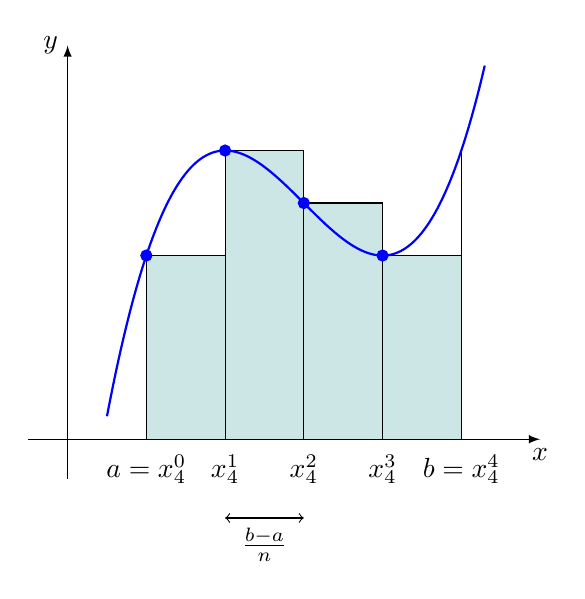
\begin{tikzpicture}[scale=1,declare function={f(\x)=((1/3)*(\x)^(3)-3*(\x)^(2)+8*\x-3;}]
\coordinate (start) at (.8,{f(.8)});
\coordinate (x0) at (1,{f(1)});
\coordinate (x1) at (2,{f(2)});
\coordinate (x2) at (3,{f(3)});
\coordinate (x3) at (4,{f(4)});
\coordinate (x4) at (5,{f(5)});
\coordinate (end) at (5.05,{f(5.05)});
\draw[fill=teal!20!white] (1,0) rectangle (2,{f(1)});
\draw[fill=teal!20!white] (2,0) rectangle (3,{f(2)});
\draw[fill=teal!20!white] (3,0) rectangle (4,{f(3)});
\draw[fill=teal!20!white] (4,0) rectangle (5,{f(4)});
\draw (5,0)--(5,{f(5)});
\draw [-latex] (-0.5,0) -- (6,0) node (xaxis) [below] {$x$};
\draw [-latex] (0,-0.5) -- (0,5) node [left] {$y$};
\foreach \x/\xtext in {1/a=x^0_{4} ,2/x^1_{4}, 3/x^2_{4} , 4/x^3_{4} , 5/b=x^4_{4}}
 \draw[xshift=\x cm] (0pt,3pt) -- (0pt,0pt) 
node[below=2pt,fill=white,font=\normalsize]
  {$\xtext$};
\draw[domain=.5:5.3,samples=200,variable=\x,blue,thick] plot ({\x},{f(\x)});                 
\foreach \n in {0,1,2,3}
\draw[blue,fill=blue] (x\n) circle (2pt) node[font=\normalsize] {$ $};    
\draw[<->] (2,-1)--(3,-1) node[below,midway] {$\frac{b-a}{n}$};      
\end{tikzpicture}
\end{marginfigure}


\section{Intégration des relations de comparaisons}
\begin{prop}{}
    Soit $f: \Rp \rightarrow \C$ une fonction continue par morceaux et $g, h:\Rp \rightarrow \Rp$ deux fonctions continues par morceaux, strictement positives. On suppose que $f = o_{+\infty}(g)$ et $f \sim_{+\infty} h$.\\
    \begin{itemize}
        \item Si $g$ et $h$ ne sont pas intégrables sur $\Rp$,
        $$\int_{0}^{x} f = o_{+\infty} \left(\int_{0}^{x} g \right) \text{ et } \int_{0}^{x} f \sim_{+\infty} \int_{0}^{x} h.$$
        \item Si $g$ et $h$ sont intégrables sur $\Rp$,
        $$\int_{x}^{+\infty} f = o_{+\infty} \left(\int_{x}^{+\infty} g \right) \text{ et } \int_{x}^{+\infty} f \sim_{+\infty} \int_{x}^{+\infty} h.$$
    \end{itemize}
\end{prop} 

La démonstration est analogue à celle de la \nameref{sommation_relations_comparaison}

\section{Transformée de \textsc{Fourier} de la loi normale}
\input{chapitres/integration/transformee_de_fourier_de_la_loi_normale}

\section{Intégrale à paramètre dans les bornes}
\begin{itemize}
    \item On pose $f:x \mapsto \int_{x}^{x^2} \frac{\d t}{\ln (t)}$.
    $$\displaystyle f(x) = \int_{x}^{x^2} \frac{t}{t \ln (t)}\ \d t \leqslant x^2 \int_{x}^{x^2} \frac{\d t}{t \ln(t)} = x^2 \bigl[ \ln (\ln (t)) \bigr]_x^{x^2} = x^2 \ln(2)$$.
\end{itemize}

\section{Intégrale de \textsc{Dirichlet}}
\textcolor{red}{A revoir}
\begin{tcolorbox}
    L'intégrale de \textsc{Dirichlet} (1829) est l'intégrale de la fonction sinus cardinal sur la demi-droite des réels positifs
    $$\int_{0}^{+\infty} \frac{\sin x}{x}\ \d x = \frac{\pi}{2}.$$
\end{tcolorbox}

\begin{enumerate}
    \item Montrer que $\int_{0}^{1} \frac{\sin (t)}{t}\ \d t$ est convergente. 
    \item Deux méthodes.
    \begin{itemize}
        \item Montrer que la série de terme général $\int_{n \pi}^{(n+1) \pi} \frac{\sin(t)}{t}\ \d t$ est convergente. En déduire que $\int_{1}^{+ \infty} \frac{\sin(t)}{t}\ \d t$ converge. 
        \begin{enumerate}
            \item Montrer que $u_n = \int_{n \pi}^{(n+1) \pi} \frac{\sin(t)}{t}\ \d t$ est le terme général d'une série alternée. Donc $\sum u_n$ converge.\\
            Attention: on ne peut pas en déduire directement que $\sum\limits_{n=0}^{+ \infty} \int_{n \pi}^{(n+1) \pi} \frac{\sin(t)}{t}\ \d t = \int_{1}^{+ \infty} \frac{\sin(t)}{t}\ \d t$ car on n'a pas encore démontrer la convergence du deuxième membre (c.f. relation de \textsc{Chasles}).\\
            \item Il faut montrer la convergence de $\int_{\pi}^{x} \frac{\sin (t)}{t}\ \d t$. \textcolor{green}{A compléter.}
        \end{enumerate}
        \item On peut aussi procéder par intégration par parties en posant
        $$
        \begin{drcases}                
            u(t) = \frac{1}{t}\\
            v(t) = - \cos(t)
        \end{drcases}
        \mathscr{C}^1 \text{ sur } [1, +\infty].
        $$
        Bien présicer que $u(t)v(t)=-\frac{\cos(t)}{t}$ admet une limite finie en 1 et en $+ \infty$.\\
        \textcolor{red}{Les IPP préservent la régularité de l'intégrale MAIS ne préservent pas l'intégrabilité.}
    \end{itemize}
    \item On en déduit immédiatement que $\int_{0}^{+ \infty} \frac{\sin (t)}{t}\ \d t$ converge.
    \item De plus, on peut montrer que cette intégrale est semi-convergente (i.e. elle n'est pas intégrable sur $\Rp$). Pour cela, montrer que pour tout entier naturel $n$, $\int_{n \pi}^{(n+1) \pi} \frac{\sin(t)}{t}\ \d t \geqslant \frac{2}{(n+1) \pi}$. 
\end{enumerate}
    
\underline{Remarque:} La fonction sinus cardinal \textbf{n'est pas intégrable} sur $\Rpe$ (cf. le prochain exercice).

\section{Intégrabilité de \texorpdfstring{$\frac{\sin(t)}{t}$ sur $\Rpe$}{sin(t)/t sur R+*}}
\begin{tcolorbox}
    La fonction sinus cardinal $\mathrm{sinc}:t \mapsto \frac{\sin(t)}{t}$ n'est pas intégrable sur $]0, +\infty[$.
\end{tcolorbox}

\begin{marginfigure}[-2.5cm]
    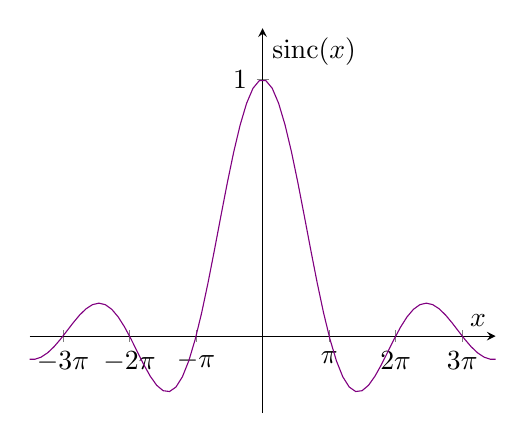
\begin{tikzpicture}
\begin{axis}[
    width=7.5cm,
    % grid=both,
    xmin=-11,
    xmax=11,
    ymin=-0.3,
    ymax=1.2,
    xlabel=$x$,
    ylabel=$\mathrm{sinc}(x)$,
    axis lines=center,
    xticklabels={$-3\pi$, $-2\pi$, $-\pi$, $\pi$, $2\pi$, $3\pi$},
    xtick={-3*3.141592, -2*3.141592, -3.141592, 3.141592, 2*3.141592, 3*3.141592},
    ytick={0, 1}
]
  \addplot[
    domain=-15:15,
    violet,
    ultra thick,
    samples=100,
  ] plot[thin] {sin(deg(x))/x};
\end{axis}
\end{tikzpicture}
\end{marginfigure}

\begin{preuve}
    On utilise le fait que pour tout $t \in \left[ \frac{\pi}{4} + k\pi, \frac{3 \pi}{4} + k \pi \right]$, $|\sin t| \geqslant \frac{1}{\sqrt{2}}$. \\
    Ainsi, pour tout $n \in \Ne$,
    \begin{align*}
        \int_{3 \pi / 4}^{n \pi + 3 \pi / 4} \left| \frac{\sin t}{t} \right| \d t &= \sum_{k=1}^n \int_{k \pi - \pi/4}^{k \pi + 3 \pi/4} \left| \frac{\sin t}{t} \right| \d t \\
        &\geqslant \frac{1}{\sqrt{2}} \sum_{k=1}^{n} \int_{k \pi - \pi/4}^{k \pi + 3 \pi/4} \frac{1}{t} \d t \\
        &\geqslant \frac{1}{\sqrt{2}} \sum_{k=1}^n \frac{\pi}{k \pi + 3 \pi/4} \\
    \end{align*}
    Or la série harmonique diverge et donc par théorème de comparaison, on obtient la non intégrabilité du sinus cardinal sur $\Rpe$.
\end{preuve}

\begin{preuve}
    Une démonstration qui ma paraît plus naturelle (\url{https://www.agreg-maths.fr/uploads/versions/1175/dirichlet.pdf}) \\
    Soit $N \in \Ne$, alors:
    \begin{align*}
        \int_0^{N \pi} \frac{|\sin x|}{x} \d x &= \sum_{k=0}^{N-1} \int_{k \pi}^{(k+1) \pi} \frac{|\sin x|}{x} \d x \\
        \text{ par changement de variable} &= \sum_{k=0}^{N-1} \int_0^\pi \frac{|\sin x|}{x + k \pi} \d x \\
        &\geqslant \sum_{k=0}^{N-1} \frac{1}{(k+1) \pi} \int_0^\pi \sin x \d x \\
        &\geqslant \frac{2}{\pi} \sum_{k=1}^N \frac{1}{k} \xrightarrow[N \to + \infty]{} + \infty.
    \end{align*}
\end{preuve}

\section{Intégrale de \textsc{Dirichlet} via une intégrale à paramètre}
Soit la transformée de \textsc{Laplace} de la fonction sinus cardinal:
$$F:x \to \int_{0}^{+ \infty} \exp(-xt) \frac{\sin (t)}{t} \d t$$
    
\begin{enumerate}
    \item \emph{Montrer que $F$ est définie sur $\Rp$.}
    \begin{itemize}
        \item Si $x > 0$, majorer l'intégrande par $t \mapsto \exp(-xt)$.
        \item Si $x = 0$, montrer le prolongement par continuité de la fonction sinus cardinal en $0$ puis intégrer la fonction sinus cardinal par parties sur $[1, +\infty]$.
    \end{itemize}
    \item \emph{Calculer $F$ sur $\Rpe$, en déduire la valeur de la fonction de \textsc{Dirichlet}}
\end{enumerate}

\section{Intégrales eulériennes}
\subsection{Fonction Gamma d'\textsc{Euler}}

\begin{marginfigure}[5cm]
    \begin{tikzpicture}[]

\begin{axis}[
xmin = -4.9, xmax = 5.1, 
%ymin = -3.5, ymax = 3.5,  
restrict y to domain=-6:6,
axis lines = middle,
axis line style={-latex},  
xlabel={$x$}, 
ylabel={$\Gamma(x)$},
%enlarge x limits={upper={val=0.2}},
enlarge y limits=0.05,
x label style={at={(ticklabel* cs:1.00)}, inner sep=5pt, anchor=north},
y label style={at={(ticklabel* cs:1.00)}, inner sep=2pt, anchor=south east},
]

\addplot[color=red, samples=222, smooth, 
domain = 0:5] gnuplot{gamma(x)};

\foreach[evaluate={\N=\n-1}] \n in {0,...,-5}{%
\addplot[color=red, samples=555, smooth,  
domain = \n:\N] gnuplot{gamma(x)};
%
\addplot [domain=-6:6, samples=2, densely dashed, thin] (\N, x);
}%
\end{axis}
\end{tikzpicture}
    \caption{Graphe de la fonction Gamma}
\end{marginfigure}

\begin{defi}
    Pour tout $x$ > 0 réel, la \emph{fonction Gamma d'\textsc{Euler}} est définie par: 
    $$\Gamma(x) \defeq \int_{0}^{+\infty} t^{x-1} \me^{-t} \d t.$$
\end{defi}

\marginnote[-2mm]{Cette fonction, introduite en 1729 par le mathématicien suisse, prolonge la fonction factorielle à l'ensemble des nombres complexes (à l'exception des entiers négatifs).}

\begin{remarque}
    À un changement de variable près, la fonction $\Gamma$ est la \nameref{transformee_laplace} de la fonction $t \mapsto t^x$. 
\end{remarque} 
\underline{Propriétés principales:}
\begin{itemize}
    \item $\Gamma$ est définie si et seulement si $x>0$.
    \item Pour tout $x > 0$, $\Gamma(x+1) = x\Gamma(x)$.
    \item En particulier, $\boxed{\forall n \in \N$, $\Gamma(n+1) = n!}$. 
\end{itemize}
\begin{preuve}
    La fonction $f:(x,t) \mapsto t^{x-1} \me^{-t}$ est continue sur $]0, + \infty[$ comme produit de fonctions qui y sont continues. La fonction $f$ est donc intégrable sur tout segment de $]0, +\infty[$. Il reste à étudier son intégrabilité en $0$ et en $+ \infty$:
    \begin{itemize}
        \item En $+\infty:$ par croissances comparées, $t^{x-1} \me^{-t} = o_{+\infty} \left(\frac{1}{t^2} \right)$. D'après le théorème de comparaison des fonctions à termes positifs, $f$ est intégrable au voisinage de $+\infty$.
        \item En $0$: $f(x,t) \sim_0 t^{x-1}$ qui est intégrable d'après \textsc{Riemann} si et seulement si $1-x < 1$ i.e. si et seulement si $\boxed{x > 0}$.
    \end{itemize}
\end{preuve}
\underline{Dérivées successives:} \\
Utiliser une domination locale sur un segment $[a, A] \subset \R_+^\star$ par la fonction:
$$\varphi_k:t \mapsto 
\begin{cases}
    |\ln t |^k \me^{-t} t^{a-1}, & \text{si } t \in ]0, 1] \\
    |\ln t |^k \me^{-t} t^{A-1}, & \text{si } t > 1
\end{cases}
$$
$$\boxed{\forall k \in \N,\ \forall x \in \R_+^\star,\ \Gamma^{(k)}(x) = \int_{0}^{+\infty} (\ln t)^k t^{x-1} \me^{-t} \d t}$$

\underline{Exercice:} \url{https://share.miple.co/content/t8BIcXSjdEslq}

\subsection{Fonction bêta}
\begin{itemize}
    \item Pour tout $(p,q) \in \N^2$, on note 
    $$I_{p,q} \defeq \int_{0}^{1} x^p (1-x)^q \d x$$
    \begin{enumerate}
        \item Déterminer une relation entre $I_{p,q}$ et $I_{p+1, q-1}$ grâce à une IPP.
        \item En déduire l'expression de $I_{p,q}$ à l'aide de factorielles.
        $$\boxed{I_{p,q} = \frac{p! q!}{(p + q + 1)!}}$$
    \end{enumerate}
\end{itemize}
\url{https://fr.wikipedia.org/wiki/Intégrale_d'Euler} \\
\cite{calcul_infinitesimal} Chapitre IV, 3 Intégrales eulériennes, page 125.


\section{Intégrale de \textsc{Gauss}}
\begin{prop}{}
    $$\int_{0}^{+\infty} \me^{-x^2} \d x = \frac{\sqrt{\pi}}{2}$$
\end{prop}

\begin{exercice}
    \marginnote[0cm]{\cite{maths-france} Planche no 13. Suites et séries d’intégrales}
    \begin{enumerate}
        \item \textbf{Première méthode:} \say{ à la main }. \\ 
        Pour $n \in \Ne$, on pose
        $$
        f_n(x) \defeq
        \begin{cases}
            \left(1 - \frac{x}{n} \right)^n &\text{si } x \in [0, n] \\
            0 &\text{si } x \geqslant n
        \end{cases}.
        $$
        Pour tout réel positif $x$, on pose $f(x) = \me^{-x^2}$.
        \begin{enumerate}
            \item Montrer que pour tout réel positif $x$, 
            $$|f(x) - f_n(x)| \leqslant \frac{1}{n \me}.$$
            \item À l'aide de la suite $(f_n)_{n \in \Ne}$, calculer l'intégrale de \textsc{Gauss}.
        \end{enumerate}
        \item \textbf{Deuxième méthode:} \say{ avec le théorème de convergence dominée }. \\
        Pour $n \in \Ne$, on pose
        $$
        f_n(x) \defeq
        \begin{cases}
            \left(1 - \frac{x^2}{n} \right)^n &\text{si } x \in [0, \sqrt{n}] \\
            0 &\text{si } x > \sqrt{n}
        \end{cases}.
        $$
        \begin{enumerate}
            \item Montrer que la suite $(f_n)_{n \in \Ne}$ converge simplement sur $\Rp$ vers la fonction $f:x \mapsto \me^{-x^2}$.
            \item À l'aide de la convergence dominée, calculer l'intégrale de \textsc{Gauss}.
        \end{enumerate}
    \end{enumerate}
\end{exercice}

\begin{solution}
\end{solution}

\section{Intégrale de \textsc{Wallis}} \label{integrale_wallis}
La page \url{https://fr.wikipedia.org/wiki/Intégrale_de_Wallis} est très complète. 

\begin{defi}{Intégrale de \textsc{Wallis}}
    $$\Wallis_n \defeq \int_{0}^{\frac{\pi}{2}} \sin^n x \d x = \int_{0}^{\frac{\pi}{2}} \cos^n x \d x$$
\end{defi}

\begin{prop}{} \labprop{prop_wallis}
    $$\Wallis_{2p} = \frac{\binom{2p}{p}}{2^{2p}}\frac{\pi}{2} \text{ et } \Wallis_{2p+1} = \frac{2^{2p} (p!)^2}{(2p+1)!}$$
    $$\Wallis_{n+1} \sim \Wallis_n \qquad \Wallis_n \sim \sqrt{\frac{\pi}{2n}}$$
    $$\Wallis_n \Wallis_{n+1} = \frac{\pi}{2(n+1)}$$
\end{prop}

\begin{preuve}
    Calculons $\Wallis_{n+2}$ en effectuant une intégration par parties. On pose $u(t) \defeq - \cos(t)$ et $v(t) \defeq \sin^{n+1}(t)$, toutes deux de classe $\mathscr{C}^1$ sur $\left[0, \frac{\pi}{2} \right]$. 
    \begin{align*}
        \Wallis_{n+2} &= \underbrace{\left[ -\cos(t) \sin^{n+1}(t) \right]_0^{\pi/2}}_{=0} + (n+1) \int_0^{\pi/2} \cos^2 (t) \sin^n(t) \d t \\
        &= (n+1) \int_0^{\pi/2} (1 - \sin^2(t)) \sin^n(t) \d t \\
        &= (n+1) \Wallis_n - (n+1) \Wallis_{n+2} \\
        \text{soit } (n+2) \Wallis_{n+2} &= (n+1) \Wallis_n.
\end{align*}
Soit $p \in \N$. D'après la relation précédente, 
\begin{figure*}[h!]
\begin{multicols}{2}
\begin{align*}
    \Wallis_{2p} &= \frac{2p-1}{2p} \Wallis_{2p-2} \\
    &= \frac{2p-1}{2p} \times \frac{2p-3}{2p-2} \times \cdots \times \frac{1}{2} \times \underbrace{\Wallis_0}_{=\pi/2} \\
    &= \frac{\prod\limits_{k=1}^p (2k+1)}{\prod\limits_{k=1}^{p+1} (2k)} \frac{\pi}{2} \\
    &= \frac{\left[\prod\limits_{k=1}^p (2k+1) \right] \times \left[ \prod\limits_{k=1}^{p+1} (2k) \right]}{\left[\prod\limits_{k=1}^{p+1} (2k) \right]^2} \frac{\pi}{2} \\
    \Wallis_{2p} &= \frac{(2p)!}{2^{2p}(p!)^2} \frac{\pi}{2}.
\end{align*}
\begin{align*}
    \Wallis_{2p+1} &= \frac{2p}{2p+1} \Wallis_{2p-1} \\
    &= \frac{2p}{2p+1} \times \frac{2p-2}{2p-1} \times \cdots \times \frac{2}{3} \times \underbrace{\Wallis_1}_{=1} \\
    &= \frac{\prod\limits_{k=1}^p (2k)}{\prod\limits_{k=0}^p (2k+1)} \\
    &= \frac{\left[ \prod\limits_{k=1}^p (2k) \right]^2}{\left[ \prod\limits_{k=0}^p (2k+1) \right] \left[ \prod\limits_{k=1}^p (2k) \right]} \\
    \Wallis_{2p+1} &= \frac{2^{2p}(p!)^2}{(2p+1)!}.
\end{align*}
\end{multicols}
\end{figure*}
\end{preuve}

\subsection{Séries génératrices}

\textcolor{red}{texte}

\begin{prop}{}
    \marginnote[0cm]{\url{https://fr.wikipedia.org/wiki/Intégrale_de_Wallis}}
    La série génératrice des termes pairs est 
    $$\sum_{p=0}^\infty \Wallis_{2p} x^{2p} = \frac{\pi}{2} \frac{1}{\sqrt{1-x^2}}.$$
    La série génératrice des termes impairs est 
    $$\sum_{p=0}^\infty \Wallis_{2p+1} x^{2p+1} = \frac{\arcsin x}{\sqrt{1-x^2}}.$$
\end{prop}

\begin{exercice}
    Soit $x \in ]0,1[$. Calculer $\sum\limits_{n=0}^\infty (-1)^n \Wallis_n$ puis $\sum\limits_{n=0}^\infty \Wallis_n x^n$.
\end{exercice}

\begin{solution}
    \marginnote[0cm]{fic00126}
    D'après \vrefprop{prop_wallis}, $\Wallis_n \sim \sqrt{\frac{\pi}{2n}}$ et la règle de \textsc{d'Alembert} fournit $R = 1$. Soit $x \in ]-1, 1[$. \\
    Pour tout $t \in \left[ 0, \frac{\pi}{2} \right]$ et tout entier naturel $n$, $|x^n \cos^n t| \leqslant |x|^n$. Comme la série numérique de terme général $|x|^n$ converge, la série de fonctions de terme général $t \mapsto x^n \cos^n t$ est normalement convergente et donc uniformément convergente sur le segment $\left[ 0, \frac{\pi}{2} \right]$. D'après le théorème d'intégration terme à terme sur un segment, 
    \begin{align*}
        \sum_{n=0}^{+ \infty} \Wallis_n x^n &= \sum_{n=0}^{+ \infty} \left[ x^n \int_0^{\pi/2} \cos^n t \d t \right] = \int_0^{\pi/2} \left( \sum_{n=0}^{+\infty} x^n \cos^n t \right) \d t \\
        &=\int_0^{\pi/2} \frac{1}{1 - x \cos t} \d t \\
        &= \int_0^1 \frac{1}{1 - x \frac{1-u^2}{1+u^2}} \frac{2}{1 + u^2} \d u \quad \text{en posant } u = \tan \frac{t}{2} \\
        &= 2 \int_0^1 \frac{1}{(1+x)u^2 + (1-x)} \d u \\
        &= 2 \times \frac{1}{1+x} \times \frac{1}{\sqrt{\frac{1-x}{1+x}}} \left[ \arctan \left( \frac{u}{\sqrt{\frac{1-x}{1+x}}} \right) \right]_0^1 \\
        \sum_{n=0}^{+ \infty} \Wallis_n x^n &= \frac{2}{\sqrt{1-x^2}} \arctan \sqrt{\frac{x+1}{x-1}}.
    \end{align*}
\end{solution}

\subsection{Calcul de l'intégrale de \textsc{Gauss}}
\marginnote[0cm]{\url{https://fr.wikipedia.org/wiki/Intégrale_de_Wallis}}
On peut aisément utiliser les intégrales de \textsc{Wallis} pour calculer l'intégrale de \text{Gauss}. \\
On utilise pour cela l'encadrement suivant, issu de la construction de la fonction exponentielle par la méthode d'\textsc{Euler}: pour tout entier $n > 0$ et tout réel $u \in ]-n, n[$, 
$$\left(1 + \frac{u}{n} \right)^n \leqslant \me^u \leqslant \left( 1 - \frac{u}{n} \right)^{-n}.$$
Posant alors $u = -x^2$, on obtient:
$$\int_0^{\sqrt{n}} \left( 1 - \frac{x^2}{n} \right)^n \d x \leqslant \int_0^{\sqrt{n}} \me^{-x^2} \d x \leqslant \int_0^{\sqrt{n}} \left( 1 + \frac{x^2}{n} \right)^{-n} \d x.$$
Or les intégrales d'encadrement sont liées aux intégrales de \textsc{Wallis}. Pour celle de gauche, il suffit de poser $x = \sqrt{n} \sin t$ ($t$ variant de $0$ à $\pi/2$). Quant à celle de droite, on peut poser $x = \sqrt{n} \tan t$ ($t$ variant de $0$ à $\pi/4$) puis majorer par l'intégrale de $0$ à $\pi/2$. On obtient ainsi:
$$\sqrt{n} \Wallis_{2n+1} \leqslant \int_0^{\sqrt{n}} \me^{-x^2} \d x \leqslant \sqrt{n} \Wallis_{2n-2}.$$
Par le théorème des gendarmes, on déduit alors de l'équivalent de $\Wallis_n$ que
$$\int_0^{+ \infty} \me^{-x^2} \d x = \frac{\sqrt{\pi}}{2}.$$

\subsection{Volume d'une boule en dimension \texorpdfstring{$n$}{n}}

\begin{exercice}
    \marginnote[0cm]{\cite{fmaalouf}}
    Pour $n \in \Ne$ et $R \in \Rpe$ on désigne par $V_n(R)$ le volume de la boule de $\R^n$ de centre $O$ et de rayon $R$, 
    $$V_n(R) \defeq \idotsint_{x_1^2 + \cdots + x_n^2 \leqslant R^2} \d x_1 \cdots \d x_n.$$
    Montrer que pour tout $p \in \Ne$, 
    $$V_{2p}(R) = \frac{\pi^p R^{2p}}{p!}.$$
\end{exercice}

\subsection{\textsc{Grain de raisin}: Produit de \textsc{Wallis}}

\begin{prop}{Produit de \textsc{Wallis}}
    $$\prod_{n=1}^{\infty} \frac{4n^2}{4n^2-1} = \frac{\pi}{2}$$
\end{prop}

\begin{preuve}
    Puisque $\Wallis_{2n} \sim \Wallis_{2n+1}$, 
    $$\lim_{n \to +\infty} \frac{\Wallis_{2n+1}}{\Wallis_{2n} / \frac{\pi}{2}} = \frac{\pi}{2}.$$
    Or d'après le calcul des intégrales de \textsc{Wallis}:
    $$\frac{\Wallis_{2n+1}}{\Wallis_{2n} / \frac{\pi}{2}} = \frac{\frac{2^{2p}(p!)^2}{(2p+1)!}}{\frac{(2p)!}{2^{2p}(p!)^2}} = \prod_{k=1}^n \frac{4k^2}{4k^2-1}.$$
\end{preuve}

\section{Théorème de \textsc{Fubini}}

\marginnote[-2mm]{Ce théorème a été démontré par le mathématicien italien Guido \textsc{Fubini} en 1907.}
\begin{theo}{\textsc{Fubini}}
    Soit $f: [a,b] \times [c, d] \to \K$ une application continue. Alors,
    $$\int_{a}^{b} \left ( \int_{c}^{d} f(x,y) \d y \right) \d x = \int_{c}^{d} \left ( \int_{a}^{b} f(x,y) \d x \right) \d y.$$
\end{theo}

\begin{marginfigure}[5cm]
    \centering
    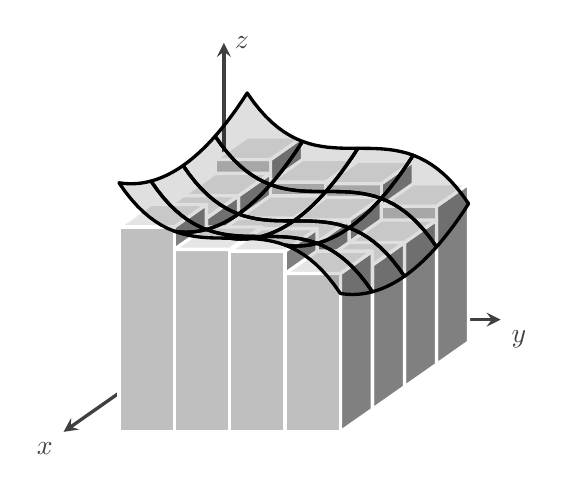
\begin{tikzpicture}[
  x=(215:2em/sqrt 2), y=(0:2em), z=(90:2em),
  declare function={f(\x,\y)=((\x-3)^2+(-\y+3)^3)/8+3;}, 
  very thick, line join=round]
\draw [-stealth, black!75] (0,0,0) -- (5,0,0) node [below left] {$x$};
\draw [-stealth, black!75] (0,0,0) -- (0,5,0) node [below right] {$y$};
\draw [-stealth, black!75] (0,0,0) -- (0,0,5) node [right] {$z$};
\foreach \x in {1,...,4}
  \foreach \y [evaluate={\j=\x+.5; \i=\y+.5; \k=f(\j,\i);}] in {1,...,4}{
    \path [fill=black!50, draw=white] (\x, \y+1, 0) -- (\x+1, \y+1, 0) -- 
      (\x+1, \y+1, \k) -- (\x, \y+1, \k) -- cycle;
    \path [fill=black!25, draw=white] (\x+1, \y, 0) -- (\x+1, \y+1, 0) -- 
      (\x+1, \y+1, \k) -- (\x+1, \y, \k) -- cycle;
    \path [fill=black!10, draw=white] (\x, \y, \k)  -- (\x+1, \y, \k) -- 
      (\x+1, \y+1, \k) -- (\x, \y+1, \k) -- cycle;
  }
 \foreach \x in {1,...,4}
   \foreach \y in {1,...,4}{
 \draw [black, fill=black, fill opacity=0.125, 
    domain=0:1, samples=10, variable=\t] 
    plot (\x+\t, \y, {f(\x+\t,\y)}) -- 
    plot (\x+1, \y+\t, {f(\x+1,\y+\t)}) -- 
    plot (\x+1-\t, \y+1, {f(\x+1-\t,\y+1)}) --
    plot (\x, \y+1-\t, {f(\x,\y+1-\t)}) -- cycle;
  }
\end{tikzpicture}
    \caption*{\centering Cette figure ne correspond pas au théorème de \textsc{Fubini}}
\end{marginfigure}

Nous allons voir la démonstration de ce résultat sous forme d'exercice.

\begin{exercice}
    Pour tout $(x, t) \in [a, b] \times [c, d]$ on pose 
    $$\varphi(x, t) \defeq \int_{a}^{x} f(u, t) \d u.$$
    \begin{enumerate}
        \item Montrer que pour tout $x \in [a, b]$, l'application $t \mapsto \varphi(x, t)$ est continue sur $[c, d]$.
        \item On pose alors, pour tout $x  \in [a, b]$ 
        $$\psi(x) \defeq \int_{c}^{d} \varphi(x, t) \d t.$$
        Montrer que $\psi$ est de classe $\mathscr{C}^1$ sur $[a, b]$, préciser $\psi'$.
        \item En déduire:
        $$\forall x \in [a, b],\ \int_{a}^{x} \left ( \int_{c}^{d} f(u,t) \d t \right) \d u = \int_{c}^{d} \left ( \int_{a}^{x} f(u,t) \d u \right) \d t.$$
    \end{enumerate}
\end{exercice}

\marginnote[0cm]{Correction du sujet Mines Maths 2 PSI 2021 par Doc Solus.} 
\begin{solution}
    \begin{enumerate}
        \item Application du théorème de continuité des intégrales à paramètre. \\
        Pour la domination : $f$ est continue sur une partie fermée bornée de $\R^2$, donc d'après le théorème des bornes, $f$ est bornée sur $[a, b] \times [c, d]$ par une constante $M \in \Rp$.
        \item Application du théorème de dérivation des intégrales à paramètre à la fonction $x \mapsto \int_{c}^{d} \varphi(x, t) \d t$:
        \begin{itemize}
            \item $\forall t \in [c, d],\ x \mapsto \varphi(x, t)$ est de classe $\mathscr{C}^1$ sur $[a, b]$ car c'est la primitive s'annulant en $a$ de la fonction continue $x \mapsto f(x, t)$. 
            \item $\frac{\partial \varphi}{\partial x}(x, t) = f(x, t)$
            \item La domination se fait par le même constante $M$ que précédemment. 
        \end{itemize}
        $$\forall x \in [a, b] \quad \psi'(x) = \int_{c}^{d} f(x, t) \d t.$$
        \item Soit $x \in [a, b]$. D'une part,
        $$\psi(x) = \int_{c}^{d} \left ( \int_{a}^{x} f(u,t) \d u \right) \d t.$$
        D'autre part, d'après la question précédente et le théorème fondamental de l'analyse, 
        \begin{align*}
            \int_{a}^{x} \left ( \int_{c}^{d} f(u,t) \d t \right) \d u &= \int_{a}^{x} \psi'(u) \d u  = \psi(x) - \psi(a) \\
            \text{Or } \psi(a) &= \int_{c}^{d} \varphi(a, t)\ \d t \\
            \text{et } \forall t \in [c, d] \quad \varphi(a, t) &= \int_{a}^{a} f(u, t) \d u = 0
        \end{align*}
        d'où $\psi(a) = 0$ et le résultat. \\
        En particulier, pour $x = b$ on obtient le résultat final.
    \end{enumerate}
\end{solution}    


\section{Transformée de \textsc{Laplace}} 
\label{transformee_laplace}
\todoinline{Rechercher l'exercice corrigé sur les théorèmes des valeurs initiales / finales.}

La transformation de \textsc{Laplace} généralise la transformation de \textsc{Fourier} qui est également utilisée pour résoudre les équations différentielles : contrairement à cette dernière, elle tient compte des conditions initiales et peut ainsi être utilisée en théorie des vibrations mécaniques ou en électricité dans l'étude des régimes forcés sans négliger le régime transitoire. De manière générale, ses propriétés vis-à-vis de la dérivation permettent un traitement plus simple de certaines équations différentielles, et elle est de ce fait très utilisée en automatique. \\
Dans ce type d'analyse, la transformation de \textsc{Laplace} est souvent interprétée comme un passage du domaine temps, dans lequel les entrées et sorties sont des fonctions du temps, dans le domaine des fréquences, dans lequel les mêmes entrées et sorties sont des fonctions de la \say{ fréquence } (complexe) $p$. Ainsi; il est possible d'analyser simplement l'effet du système sur l'entrée pour donner la sortie en matière d'opérations algébriques simples (cf. théorie des fonctions de transfert en électronique ou en mécanique). 

\begin{defi}{Transformée de \textsc{Laplace}}
    Pour tout fonction $f \in \mathscr{C}(\Rp, \R)$, on note, lorsqu'elle converge, 
    $$\mathscr{L}(f)(p) \defeq \int_{0}^{+ \infty} \e^{-pt} f(t) \d t.$$
    La fonction $\mathscr{L}(f)$ est la \emph{transformée de \textsc{Laplace} de f}.
\end{defi}

\marginnote[0cm]{Sources : \cite{exos_oraux} + \cite{acamanes} (Exercice cerise Ch. 12)}
\underline{Démonstration du théorème de la valeur finale:}
\begin{itemize}
    \item Généralisation classique du théorème des bornes $\leadsto$ $f$ est bornée
    \item Changement de variable: $\varphi: u \mapsto \frac{u}{p}$
    \item Caractérisation séquentielle de la limite
    \item Théorème de convergence dominée
\end{itemize}

